\documentclass[conference]{IEEEtran}
\IEEEoverridecommandlockouts
% The preceding line is only needed to identify funding in the first footnote. If that is unneeded, please comment it out.
\usepackage{cite}
\usepackage{amsmath,amssymb,amsfonts}
\usepackage{algorithmic}
\usepackage{graphicx}
\usepackage{hyperref}
\usepackage{textcomp}
\usepackage{xcolor}
\def\BibTeX{{\rm B\kern-.05em{\sc i\kern-.025em b}\kern-.08em
    T\kern-.1667em\lower.7ex\hbox{E}\kern-.125emX}}

\hypersetup{
    colorlinks=true,
    linkcolor=blue,
    filecolor=magenta,
    urlcolor=cyan,
}

\begin{document}

\title{Machine Learning Project Report}

\author{
\IEEEauthorblockN{Rodrigo Castiel}
\IEEEauthorblockA{\textit{Center for Informatics} \\
\textit{Federal University of Pernambuco}\\
Recife, Brazil \\
rcrs2@cin.ufpe.br}
}


\maketitle

\begin{abstract}
In the first part of this report, we compare $k$-means to KCM-F-GH, its hard clustering variation in feature space proposed by Cunha et al \cite{??}.
Both methods are evaluated on the segmentation dataset available in \cite{??} by 
computing the adjusted rand index to analyze the similarity between the predicted cluster solutions and the ground-truth labels.
In the second part, we perform a comparative analysis between three classifiers: a maximum likelihood gaussian estimator, a $k$-nearest neighbors classifier and a hybrid-model committee classifier.
Those classifiers are also tested on the segmentation dataset.
We run cross-validation multiple times to estimate the accuracy and the error margin of each classifier.
At the end, we perform Friedman test to determine the best algorithm.
Our results show that KCM-F-GH outperforms the standard $k$-means in most cases, with the tradeoff of being considerably more time-consuming.
In the second part, our experiments show that both KNN and the hybrid classifier are equally accurate in the dataset, and better than the maximum-likelihood estimator.


\end{abstract}

\begin{IEEEkeywords}
clustering, supervised learning, classification, pattern recognition
\end{IEEEkeywords}

\section{Introduction}
This research report contains two main sections.
The first one briefly describes how $k$-means and KCM-F-GH were implemented, and how they performed in the experiments.
In the second one, we point some implementation strategies for the maximum likelihood gaussian estimator (MLE), the $k$-nearest neighbors classifier (KNN) and the hybrid-model committee classifier. Then, we compare their accuracy in a series of experiments.

The \textit{Python} code, the development history and the dataset are all available on Rodrigo Castiel's personal github (click \href{https://github.com/RodrigoCastiel/am_f}{here}).
Basic repository structure:
\begin{itemize}
\item \textit{part\_1.py}: main script for running and comparing the clustering algorithms.
\item \textit{part\_2.py}: main script for running and comparing the supervised classifiers.
\item \textit{classifiers}: contains a list of classes, each implementing a classifier or a clustering algorithm.
\item \textit{core}: contains \textit{data\_loader.py}, a utility module for managing the segmentation data.
\item \textit{data}: training and test datasets.
\end{itemize}

Additionally, we use \textit{Numpy} and \textit{Scikit}, \textit{Python} libraries for linear algebra, statistics and learning utilities.

\section{Part I - Clustering}

\subsection{Implementation}

The test code start point is located in \textit{part\_1.py}.
The script arguments, to be passed in from the terminal, are a list of views which will be tested.
For example the list \textit{RGB} and \textit{SHAPE} tells the program to run both $k$-means and KCM-F-GH on the RGB and the shape view, separately.
For each view, the script then builds each classifier and calls the method fit on it.
The parameter $num\_times$ controls how many times KCM-F-GH will be executed before the best fit run is taken.
The implementation of $k$-means and KCM-F-GH are located in \textit{k\_means\_clustering.py} and \textit{kcm\_f\_gh\_clustering.py}, respectively.
They are both thoroughly documented.

\textbf{Note}. During the initial tests of KCM-F-GH, we noticed that the update of the hyper-width parameters is not robust to constant-valued features.
That is, if at a given moment a specific feature becomes constant within each cluster, the denominator of equation (24) becomes $0$ \cite{??}, which breaks the execution.
It means that before actually running this algorithm in feature space, we must remove redudant dimensions in the dataset.
For this reason, we removed the features "REGION-PIXEL-COUNT" and "SHORT-LINE-DENSITY-2" from the shape view.

\subsection{Experiments and Results}

In the first experiments, we noticed that KCM-F-GH takes an average of approximately one hour to converge on the test dataset containing $2100$ points.
Since our personal computer's hardware is not powerful, executing KCM-F-GH $100$ times per view is impossible in practice.
Instead, we run it only $10$ times per view.

\begin{figure}
\label{part_i_full}
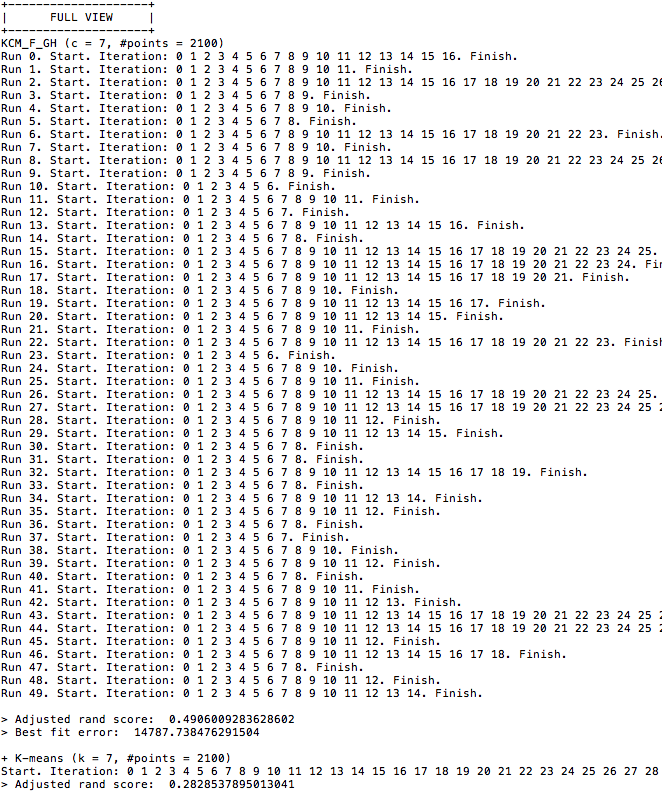
\includegraphics[width=0.50\textwidth]{part_i_full.png}
\caption{Output log of Part I on full view (RGB + shape). We run KCM-F-GH $num\_times = 50$ with random initial representatives in each cluster. Then, we pick the best fitting KCM-F-GH and compute its adjusted rand index (see bottom). KCM-F-GH achieved $0.4906$ while $k$-means achieved $0.2826$.}
\end{figure}

\section{Part II - Supervised Learning}

\subsection{Implementation}

The test code start point is located in \textit{part\_2.py}.
In the first moment, we perform a grid search in the training dataset to find the best hyper-parameters for the classifiers.
Then, we run cross-validation multiple times in the training dataset to estimate the accuracy (and its standard deviation) for each classifier.
After that, we run the classifiers on the test dataset to evaluate the overall accuracy.
Last, we perform the Friedman test to compare all pairs of classifiers.
The program writes the output log into \textit{part\_2\_log.txt}.

Each classifier contains two main methods: \textit{fit} and \textit{predict}.
\begin{itemize}
\item \textit{gaussian\_mle.py}: defines class \textit{GaussianMLE}.
In its method \textit{fit}, the training dataset is split up into subsets sharing the same label.
Then, the gaussian distribution parameters (\textit{i.e.}, the mean $\mu$ and the covariance matrix $\Sigma$) are estimated for each class.
Once trained, the MLE classifier is also able to compute the a posteriori probabilities for a given point.
This is needed for the hybrid classifier.
\item \textit{knn\_classifier.py}: defines class \textit{KNNClassifier}.
It performs no computation in the method \textit{fit}.
Instead, it only stores the labeled points.
In the method \textit{predict}, we then compute the distances from each input point to all examples and use a heap to keep track of the nearest $k$ points.
The predicted label is computed by picking the class of the majority.
\item \textit{combinex\_max\_classifier.py}: defines class \textit{CombinedMaxClassifier}, the hybrid classifier.
It takes a list of views to be tested on the dataset, and the hyper-parameter $k$ for its KNN classifiers.
Internally, it performs a cartesian product between the list of classifiers (MLE and KNN) and all views.
It forwards \textit{fit} and \textit{predict} to all its classifier-view pairs, and returns the combined answer.

\end{itemize}

\subsection{Experiments and Results}

\begin{figure}
\label{part_ii_results}
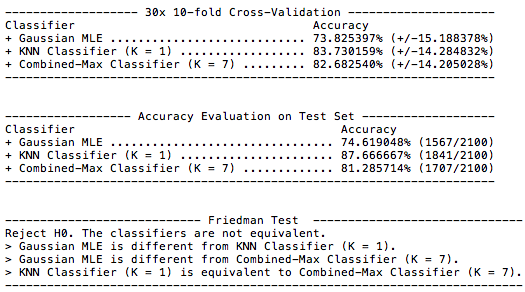
\includegraphics[width=0.45\textwidth]{part_ii_results.png}
\caption{Output log of Part II. The first section shows the average accuracy and its error margin measured by running 10-fold cross-validation 30 times on the training dataset. The second section shows the overall accuracy measured on the test dataset. The last section shows the Friedman test result (on the training dataset).}
\end{figure}

Figure \ref{part_ii_results} was taken from the output log of Part II.
Grid-search finds that the best hyper-parameters are $k = 1$ for KNN and $k = 7$ for the hybrid method.
As we can see in the cross-validation table, Gaussian MLE has the lowest accuracy among all classifiers ($\approx74\%$), while both hybrid and KNN achieve similar accuracies ($\approx 83\%$).
On the complete test set containing $2100$ points, KNN achieves the highest accuracy, followed by hybrid and then Gaussian MLE.
In fact according to the Friedman test results, KNN and hyrid are statistically equivalent.

When it comes to the comparative computational costs, KNN is certainly cheaper than hybrid, since hybrid needs to run multiple classifiers internally before combining their answers.
Gaussian MLE is indeed the cheapest method, because its prediction consists only of simple likelihood computations.

\section{Conclusion}

blah blah blah blah blah blah.

\section*{References}

Please number citations consecutively within brackets \cite{b1}. The 
sentence punctuation follows the bracket \cite{b2}. Refer simply to the reference 
number, as in \cite{b3}---do not use ``Ref. \cite{b3}'' or ``reference \cite{b3}'' except at 
the beginning of a sentence: ``Reference \cite{b3} was the first $\ldots$''

Number footnotes separately in superscripts. Place the actual footnote at 
the bottom of the column in which it was cited. Do not put footnotes in the 
abstract or reference list. Use letters for table footnotes.

Unless there are six authors or more give all authors' names; do not use 
``et al.''. Papers that have not been published, even if they have been 
submitted for publication, should be cited as ``unpublished'' \cite{b4}. Papers 
that have been accepted for publication should be cited as ``in press'' \cite{b5}. 
Capitalize only the first word in a paper title, except for proper nouns and 
element symbols.

For papers published in translation journals, please give the English 
citation first, followed by the original foreign-language citation \cite{b6}.

\begin{thebibliography}{00}
\bibitem{b1} G. Eason, B. Noble, and I. N. Sneddon, ``On certain integrals of Lipschitz-Hankel type involving products of Bessel functions,'' Phil. Trans. Roy. Soc. London, vol. A247, pp. 529--551, April 1955.
\bibitem{b2} J. Clerk Maxwell, A Treatise on Electricity and Magnetism, 3rd ed., vol. 2. Oxford: Clarendon, 1892, pp.68--73.
\bibitem{b3} I. S. Jacobs and C. P. Bean, ``Fine particles, thin films and exchange anisotropy,'' in Magnetism, vol. III, G. T. Rado and H. Suhl, Eds. New York: Academic, 1963, pp. 271--350.
\bibitem{b4} K. Elissa, ``Title of paper if known,'' unpublished.
\bibitem{b5} R. Nicole, ``Title of paper with only first word capitalized,'' J. Name Stand. Abbrev., in press.
\bibitem{b6} Y. Yorozu, M. Hirano, K. Oka, and Y. Tagawa, ``Electron spectroscopy studies on magneto-optical media and plastic substrate interface,'' IEEE Transl. J. Magn. Japan, vol. 2, pp. 740--741, August 1987 [Digests 9th Annual Conf. Magnetics Japan, p. 301, 1982].
\bibitem{b7} M. Young, The Technical Writer's Handbook. Mill Valley, CA: University Science, 1989.
\end{thebibliography}

\end{document}
